% Copyright 2004 by Till Tantau <tantau@users.sourceforge.net>.
%
% In principle, this file can be redistributed and/or modified under
% the terms of the GNU Public License, version 2.
%
% However, this file is supposed to be a template to be modified
% for your own needs. For this reason, if you use this file as a
% template and not specifically distribute it as part of a another
% package/program, I grant the extra permission to freely copy and
% modify this file as you see fit and even to delete this copyright
% notice. 


\documentclass{beamer}
\usepackage{mathtools}
% There are many different themes available for Beamer. A comprehensive
% list with examples is given here:
% http://deic.uab.es/~iblanes/beamer_gallery/index_by_theme.html
% You can uncomment the themes below if you would like to use a different
% one:
%\usetheme{AnnArbor}
%\usetheme{Antibes}
%\usetheme{Bergen}
%\usetheme{Berkeley}
\usetheme{Berlin}
%\usetheme{Boadilla}
%\usetheme{boxes}
%\usetheme{CambridgeUS}
%\usetheme{Copenhagen}
%\usetheme{Darmstadt}
%\usetheme{default}
%\usetheme{Frankfurt}
%\usetheme{Goettingen}
%\usetheme{Hannover}
%\usetheme{Ilmenau}
%\usetheme{JuanLesPins}
%\usetheme{Luebeck}
% \usetheme{Madrid}
%\usetheme{Malmoe}
%\usetheme{Marburg}
%\usetheme{Montpellier}
%\usetheme{PaloAlto}
%\usetheme{Pittsburgh}
%\usetheme{Rochester}
%\usetheme{Singapore}
%\usetheme{Szeged}
%\usetheme{Warsaw}

\title{Understanding how Ideas Spread over Twitter using Epidemiological Models} 

% A subtitle is optional and this may be deleted
\subtitle{Presentation}

\author{B.~Adishaa \and F.~Vermehr \and Q. ~Vilchez}
% - Give the names in the same order as the appear in the paper.
% - Use the \inst{?} command only if the authors have different
%   affiliation.

\institute[University of Toronto] % (optional, but mostly needed)
{
  MAT482 Topics in Mathematics: Math Models\\
  University of Toronto}
% - Use the \inst command only if there are several affiliations.
% - Keep it simple, no one is interested in your street address.

\date{}
% - Either use conference name or its abbreviation.
% - Not really informative to the audience, more for people (including
%   yourself) who are reading the slides online

\subject{Mathematical Models}
% This is only inserted into the PDF information catalog. Can be left
% out. 

% If you have a file called "university-logo-filename.xxx", where xxx
% is a graphic format that can be processed by latex or pdflatex,
% resp., then you can add a logo as follows:

% \pgfdeclareimage[height=0.5cm]{university-logo}{university-logo-filename}
% \logo{\pgfuseimage{university-logo}}

% Delete this, if you do not want the table of contents to pop up at
% the beginning of each subsection:
\AtBeginSubsection[]
{
  \begin{frame}<beamer>{Outline}
    \tableofcontents[currentsection,currentsubsection]
  \end{frame}
}

% Let's get started
\begin{document}

\begin{frame}
  \titlepage
\end{frame}

\begin{frame}{Outline}
  \tableofcontents
  % You might wish to add the option [pausesections]
\end{frame}

% Section and subsections will appear in the presentation overview
% and table of contents.
\section{Introduction}

\begin{frame}{Introduction}
\begin{itemize}
    \item \textbf{Model:} We will use a compartment model similar to the SEIZ model (Susceptibles Exposed Infectives Skeptics) in order to describe how stories spread on Twitter. We will divide the susceptible population into $2$:{\begin{itemize}
        \item $S_1$: susceptible population which has not been infected by 'similar' topics in the past.
        \item $S_2$: susceptible population which has been infected by 'similar' topics in the past.
    \end{itemize}}
    \item \textbf{Goal:} Determine to what extent having a good understanding of $S_2$ (size, contact rates, etc) can help us better model and potentially predict how an idea will spread on Twitter.
    {\begin{itemize}
        \item \textbf{Possible Applications:} Marketing analysis, rumor detection. 
    \end{itemize}}
\end{itemize}
\end{frame}

\section{Related Work}

% You can reveal the parts of a slide one at a time
% with the \pause command:
\begin{frame}{Bettencourt et al.}
  \begin{itemize}
  \item {
    In their paper Bettencourt et al. developped the SEIZ model to describe the adoption of the Feynman diagrams by the scientific community around the world. This model introduced an exposed state and a skeptic state.
    {\begin{itemize}
        \item $Z$: The skeptic state describes a part of the population that does not believe in the the information and will not react to it.
        \item $E$: The exposed state accounts for the part of the population which have been exposed to the information but takes some time before they begin to believe/react to it.
    \end{itemize}}
    \pause % The slide will pause after showing the first item
  }
  \item {In this paper, they showed that the SEIZ model was the one that was able to best capture the dynamics in the spread of the Feynmann diagrams across the scientific community. Out of the different epidemiological models they tested, this one yielded the best fits.
   }
  \end{itemize}
\end{frame}

\begin{frame}{Fang Jin et al.}
    \begin{itemize}
        \item {In their paper, Fang Jin et al. were able to describe how news and rumors spread on twitter using the SEIZ model, and were able to observe that the SEIZ was once again the model that yielded the best fit compared to other models. 
        \pause % The slide will pause after showing the first item
        }
        \item Their results also allowed them to define a ratio $R_{SI}$, which they believe can measure how likely a story is to be a rumor or a true story.
    \end{itemize}
\end{frame}
\section{Our Approach}
\begin{frame}{SEIZ model (equations)}
\begin{equation} 
\begin{split}
\frac{dS}{dt} &= -{\beta} S\frac{I}{N} - b S\frac{Z}{N}\\
\frac{dE}{dt} &= {\beta} (1-p) S\frac{I}{N} + b(1-l)S\frac{Z}{N} - \rho E\frac{I}{N} - \epsilon E\\
\frac{dI}{dt} &= {\beta} pS\frac{I}{N}+ \epsilon E + \rho E\frac{I}{N}\\
\frac{dZ}{dt} &=  b lS\frac{Z}{N}
\end{split}
\end{equation}
\begin{align*}
 N& = S + E + Z + I   & 0\leq m<p\leq 1\\
0&\leq l \leq 1  & \frac{dN}{dt}&=0
\end{align*}


    
\end{frame}

\begin{frame}{SEIZ model (graph)}
\center
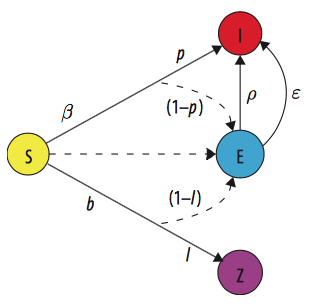
\includegraphics[width=.6\textwidth]{graphSEIZ.png}
    
\end{frame}

\begin{frame}{Modified SEIZ (equations)}
\begin{equation} 
\begin{split}
\frac{dS_1}{dt} &= -{\beta}_1 S_1\frac{I}{N} -\gamma S_1\frac{Z}{N}\\
\frac{dS_2}{dt} &= -{\beta}_2 S_2\frac{I}{N}\\
\frac{dE}{dt} &= {\beta}_1 pS_1\frac{I}{N} + {\beta}_2 mS_2\frac{I}{N} + \gamma       lS_1\frac{Z}{N} - \mu E\frac{I}{N} - \epsilon E\\
\frac{dI}{dt} &= {\beta}_1 (1-p)S_1\frac{I}{N} + {\beta}_2 (1-m)S_2\frac{I}{N} + \epsilon E + \mu E\frac{I}{N}\\
\frac{dZ}{dt} &=  \gamma (1-l)S_1\frac{Z}{N}
\end{split}
\end{equation}
with,
$$\frac{dN}{dt}&=0  \quad \text{and}\quad m,p,l \in [0,1] \quad \text{with}\quad m<p$$   
\end{frame}

\begin{frame}{Modified SEIZ (graph)}
\center
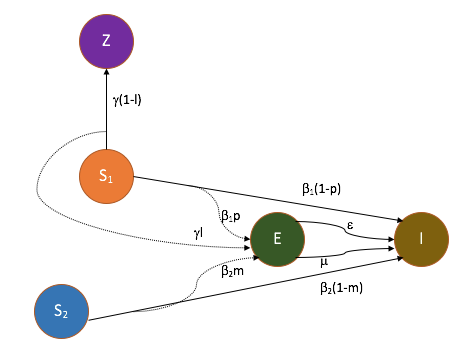
\includegraphics[width=.7\textwidth]{graphS1S1EIZ.png}
    
\end{frame}
\begin{frame}{Blocks}
\begin{block}{Block Title}
You can also highlight sections of your presentation in a block, with it's own title
\end{block}
\begin{theorem}
There are separate environments for theorems, examples, definitions and proofs.
\end{theorem}
\begin{example}
Here is an example of an example block.
\end{example}
\end{frame}

% Placing a * after \section means it will not show in the
% outline or table of contents.
\section*{Summary}

\begin{frame}{Summary}
  \begin{itemize}
  \item
    The \alert{first main message} of your talk in one or two lines.
  \item
    The \alert{second main message} of your talk in one or two lines.
  \item
    Perhaps a \alert{third message}, but not more than that.
  \end{itemize}
  
  \begin{itemize}
  \item
    Outlook
    \begin{itemize}
    \item
      Something you haven't solved.
    \item
      Something else you haven't solved.
    \end{itemize}
  \end{itemize}
\end{frame}



% All of the following is optional and typically not needed. 
\appendix
\section<presentation>*{\appendixname}
\subsection<presentation>*{For Further Reading}

\begin{frame}[allowframebreaks]
  \frametitle<presentation>{For Further Reading}
    
  \begin{thebibliography}{10}
    
  \beamertemplatebookbibitems
  % Start with overview books.

  \bibitem{Author1990}
    A.~Author.
    \newblock {\em Handbook of Everything}.
    \newblock Some Press, 1990.
 
    
  \beamertemplatearticlebibitems
  % Followed by interesting articles. Keep the list short. 

  \bibitem{Someone2000}
    S.~Someone.
    \newblock On this and that.
    \newblock {\em Journal of This and That}, 2(1):50--100,
    2000.
  \end{thebibliography}
\end{frame}

\end{document}


